
\documentclass{sig-alternate}
  \pdfpagewidth=8.5truein
  \pdfpageheight=11truein

\usepackage{cite}
\usepackage{graphicx}
\usepackage{listings}
%\usepackage{pxfonts}
\usepackage{times}
%\usepackage{xspace}
\usepackage{booktabs}
\usepackage{fancybox}
\usepackage{color}
\usepackage{multirow}
\usepackage{array}
\usepackage{tabularx}
\usepackage{url}
\urlstyle{same}
\usepackage{xcolor}
\usepackage{pgfplots}
\usepackage{tikz}
\usepackage{caption}
\usetikzlibrary{shapes,arrows, positioning}
\usetikzlibrary{patterns}
\usepackage[numbers]{natbib} % Used to fix formatting issue.
\usepackage{soul} % Needed for wrapping of highlighted text
\usepackage{balance} % Used to balance out the columns



%%% Used to anonymoyze paper
\newif\ifisnopii
%\isnopiitrue % change to true/false to remove personally identifiable information (pii)
\isnopiifalse


\definecolor{bblue}{HTML}{4F81BD}
\definecolor{rred}{HTML}{C0504D}
\definecolor{ggreen}{HTML}{9BBB59}
\definecolor{ggrey}{HTML}{707070}

% Define flow chart styles
%\tikzstyle{decision} = [diamond, draw, fill=blue!20,
%    text width=15em, text badly centered, node distance=3cm, inner sep=0pt]



\tikzstyle{block} = [rectangle, draw, fill=blue!20,
    text width=15em, text centered, rounded corners, minimum height=4em]
\tikzstyle{line} = [draw, -latex']


\lstset{ %
language=,                % choose the language of the code
basicstyle=\small,       % the size of the fonts that are used for the code \footnotesize
%numbers=left,                   % where to put the line-numbers
numberstyle=\footnotesize,      % the size of the fonts that are used for the line-numbers
stepnumber=1,                   % the step between two line-numbers. If it is 1 each line will be numbered
numbersep=5pt,                  % how far the line-numbers are from the code
backgroundcolor=\color{white},  % choose the background color. You must add \usepackage{color}
showspaces=false,               % show spaces adding particular underscores
showstringspaces=false,         % underline spaces within strings
showtabs=false,                 % show tabs within strings adding particular underscores
%frame=single,           % adds a frame around the code
tabsize=2,          % sets default tabsize to 2 spaces
captionpos=b,           % sets the caption-position to bottom
breaklines=true,        % sets automatic line breaking
breakatwhitespace=false,    % sets if automatic breaks should only happen at whitespace
escapeinside={\%*}{*)}          % if you want to add a comment within your code
}


\newcommand{\todo}[1]{\textcolor{cyan}{\textbf{[#1]}}}
\newcommand{\sam}[1]{\textcolor{red}{{\it [Sam says: #1]}}}
\newcommand{\dan}[1]{\textcolor{blue}{{\it [Dan says: #1]}}}





\makeatletter
\newenvironment{btHighlight}[1][]
{\begingroup\tikzset{bt@Highlight@par/.style={#1}}\begin{lrbox}{\@tempboxa}}
{\end{lrbox}\bt@HL@box[bt@Highlight@par]{\@tempboxa}\endgroup}

\newcommand\btHL[1][]{%
  \begin{btHighlight}[#1]\bgroup\aftergroup\bt@HL@endenv%
}
\def\bt@HL@endenv{%
  \end{btHighlight}%
  \egroup
}
\newcommand{\bt@HL@box}[2][]{%
  \tikz[#1]{%
    \pgfpathrectangle{\pgfpoint{1pt}{0pt}}{\pgfpoint{\wd #2}{\ht #2}}%
    \pgfusepath{use as bounding box}%
    \node[anchor=base west, fill=orange!30,outer sep=0pt,inner xsep=1pt, inner ysep=0pt, rounded corners=3pt, minimum height=\ht\strutbox+1pt,#1]{\raisebox{1pt}{\strut}\strut\usebox{#2}};
  }%
}
\makeatother

\lstdefinestyle{ConcolicOutput}{
   % language={SQL},basicstyle=\ttfamily,
    moredelim=**[is][\btHL]{`}{`},
   % moredelim=**[is][{\btHL[fill=green!30,draw=red,dashed,thin]}]{@}{@},
}



\begin{document}
%
% --- Author Metadata here ---
\conferenceinfo{SAC'15}{April 13-17, 2015, Salamanca, Spain.}
\CopyrightYear{2015} % Allows default copyright year (2002) to be over-ridden - IF NEED BE.
\crdata{X-XXXXX-XX-X/XX/XX}  % Allows default copyright data (X-XXXXX-XX-X/XX/XX) to be over-ridden.
% --- End of Author Metadata ---

\title{Examining the Effectiveness of Using Concolic Analysis to Detect Code Clones}
\numberofauthors{1} %  in this sample file, there are a *total*
% of EIGHT authors. SIX appear on the 'first-page' (for formatting
% reasons) and the remaining two appear in the \additionalauthors section.
%
\ifisnopii % turn on/off pii
\author{
%
% 1st. author
\alignauthor
Daniel E. Krutz and Samuel A. Malachowsky\\ 	
	\affaddr{Software Engineering Department}\\
       \affaddr{Rochester Institute of Technology}\\
       \affaddr{1 Lomb Memorial Drive}\\
       \affaddr{Rochester, NY 14623} \\
       \email{\{dxkvse, samvse\}@rit.edu}
} % Must not be a space above this
\else % turn on/off pii
\author{
\alignauthor
XXX X XXX\\
       \affaddr{xxxxx}\\
       \affaddr{xxxx, xx, xxx}\\
       \email{xxxxx@xxx.xxx}
}
\fi % end turn on/off pii

\maketitle
\begin{abstract}
During the initial construction and subsequent maintenance of an application, duplication of functionality is common, whether intentional or otherwise. This replicated functionality, known as a code clone, has a diverse set of causes and can have moderate to severe adverse effects on a software project in a variety of ways. A code clone is simply defined as multiple code fragments that produce similar results when provided the same input. While there are an array of powerful clone detection tools, most suffer from a variety of drawbacks including, most importantly, the inability to accurately and reliably detect all four types of clones.

This paper presents a new method for detecting code clones based on concolic analysis, which uses a mixture of concrete and symbolic values to traverse a large and diverse portion of the source code. By performing concolic analysis on the targeted source code and then examining the holistic output for similarities, code clone candidates can be consistently identified. We found that concolic analysis was able to accurately and reliably discover all four types of code clones with an average precision of .8, recall of .91, F-score of .85 and an accuracy of .99.

\end{abstract}


% I think this is the most appropriate
%\ccsdesc[500]{Security and privacy~Software and application security}
\category{D.2.7}{Software Engineering}Maintenance;
%They are here: http://www.acm.org/about/class/ccs98-html


%%% This was left out by 2/3 printed examples, so it may not be a bad idea to leave it out as well
%%%     Also saves space.
%\terms{xxx, xxx, xxx}


\keywords{Code Clones, Concolic Analysis, Software Engineering}



% Add in categories and keywords


\section{Introduction}
Software must continually change in order to keep up with user requirements, enhance its functionality, fix bugs, or repair security vulnerabilities. Prior work has shown that these code changes often result in cloned code for a variety of reasons. In many instances, developers knowingly duplicate functionality across the software system because of laziness or an unwillingness to refactor and retest the modified portion of the application. Careful developers know to avoid code clones and may not be aware that identical functionality exists in their system, and may on occasion unintentionally inject clones into their application~\cite{Duala-Ekoko:2010:CRD:1767751.1767754,Baker:1995:FDN:832303.836911}. Whatever the reason, clones continue to be extremely widespread in software development; estimates have shown that clones typically amount up to 30\% of an application's source code \cite{Baxter:1998:CDU:850947.853341,Kim:2005:ESC:1095430.1081737}.

Many previous works have stated that code clones are undesirable because they often lead to more bugs and make their remediation process more difficult and expensive~\cite{Duala-Ekoko:2010:CRD:1767751.1767754,Baker:1995:FDN:832303.836911,Baxter:1998:CDU:850947.853341}. Clones may also substantially raise the maintenance costs associated with an application~\cite{Juergens:2009:CCM:1555001.1555062}, the importance of which is highlighted by the fact that the maintenance phase of a software project has been found to typically comprise at least 50\% of the cost of a software project~\cite{SMR:SMR225}. Inconsistent bug fixes to cloned code across a software system increases the likeliness of further system faults~\cite{Deissenboeck_2010}.


%Ultimately, unintentionally making inconsistently applied bug fixes to cloned code across a software system increases the likeliness of further system faults~\cite{Deissenboeck_2010}.
 
 
% constitute between 40\% and 90\% of its total cost~\cite{Shukla:2008:ESM:1342211.1342232,Ducasse:1999:LIA:519621.853389,SMR:SMR225,Ueda:2002:GMS:823457.824039,Boehm:2001:SDR:619059.621640,Erlikh:2000:LLS:612986.613032}. 
 


We define the four types of code clones using the definitions from Roy et al.~\cite{Roy:2009:CEC:1530898.1531101}. Type-1 clones are the simplest, representing identical code except for variations in whitespace, comments, and layout. Type-2 clones have variations in identifiers, types, whitespace, literals, layout, and comments, but are otherwise syntactically identical. Type-3 clones are fragments which are copied and have modifications such as added or removed statements, variations in literals, identifiers, whitespace, layout and comments. Type-4 clones, the most difficult to detect, are code segments that perform the same computation, but have been implemented using different syntactic variants.

In assisting software practitioners, clone detection tools have been indispensable in detecting and managing clone-related bugs and even security vulnerabilities in software systems~\cite{Dang:2012:XTC:2420950.2421004}. Of the numerous clone detection tools, most have only been able to detect the simpler clones: type-1, type-2, and type-3. To the best of our knowledge, only a few techniques are able to detect type-4 clones, the most complicated of the four~\cite{Roy:2009:CEC:1530898.1531101}.


%MeCC, capable of reliably detecting type-4 clones, suffers from several drawbacks, including the ability to only analyze pre-processed C programs~\cite{Kim:2011:MMC:1985793.1985835}.

In this paper, we examine the effectiveness of using concolic analysis to detect code clones. Concolic analysis combines concrete and symbolic values in order to traverse all possible paths of an application (up to a given length). Traditionally used in software testing to find application faults~\cite{Kiezun:2013:HSW:2377656.2377662}, concolic analysis forms the basis of a powerful clone detection tool because it only considers the functionality of the source code and not its syntactic properties. Because of this, elements that are challenging for existing clone detection systems such as comments and naming conventions do not affect concolic analysis and its detection of clones. This research is important because any technique which can effectively discover all four types of code clones is important since so few clone detection techniques are able to do so. \\ \\ \\ \\ 

% RQs.
Our study will answer the following research questions:

\textbf{RQ1:}~\emph{What types of clones is concolic analysis effective at detecting?}\\
We find concolic analysis is able to detect all four types of clones in both a small environment and a larger clone oracle.

%% In the final release, change this to be more personable -- Refer to us not Krutz
\textbf{RQ2:}~\emph{How effective is concolic analysis for code clone detection?}\\
We measured the precision, recall, accuracy, and F-score of concolic analysis for code clone detection against two small existing oracles created by Krawitz~\cite{Kraw2012} and Roy~et al.~\cite{Roy:2009:CEC:1530898.1531101} and a larger one built by Krutz and Le~\cite{Krutz:2014:CCO:2597073.2597127}. We found that concolic analysis was able to discover clones with an average precision of .8, recall of .91, F-score of .85 and an accuracy of .99. We also found that concolic analysis for clone detection compares favorably against a robust clone detection tool, MeCC~\cite{Kim:2011:MMC:1985793.1985835}. 

In the rest of the paper, we describe how concolic analysis finds code clones, explain the types of clones it is capable of finding, and compare this technique against a leading clone detection tool.


%The remainder of the paper is organized as follows: Section~\ref{sec: howconcolicworks} describes how concolic analysis may be used to to detect software clones. Section~\ref{sec: evaluation} evaluates the ability of concolic analysis in identifying clones in relation to existing tools. Section~\ref{sec: relatedworks} discusses related works in clone detection and concolic analysis. Section~\ref{sec: threats} details some threats to the findings of this work. Section~\ref{sec: futurework} discusses future work while Section~\ref{sec: conclusion} provides concluding remarks.


\vspace{-0.08in}
\section{How Concolic Clone Detection Works}
\label{sec: howconcolicworks}


%\ifisnopii Concolic Code Clone Detection (CCCD)\cite{wcre2013}\else xxxxx \fi is a fully functional tool of our creation which uses concolic analysis for clone detection. First, concolic analysis is performed on the target application using CREST~\footnote{https://github.com/jburnim/crest}. Next, a Java component uses CTAGS~\footnote{http://ctags.sourceforge.net} to break up the concolic output at the method level. Once this is complete, a comparison process uses the Levenshtein-distance-based measurement to evaluate the similarity between the concolic output files. Finally, a report displays the detected code clone candidates. This tool, installation instructions, and further details is located on our project website\footnote{\ifisnopii\url{http://www.se.rit.edu/~dkrutz/CCCD/}\else hidden to anonymize paper\fi}.

%\subsection{Motivating Example}
Concolic code clone detection is comprised of two primary phases. An overview of this approach is shown in Figure~\ref{fig:comprocess}. The first step is the generation of the concolic output on the target application. This may be done using an existing concolic analysis tool such as Crest~\footnote{http://code.google.com/p/crest}, CATG~\footnote{https://github.com/ksen007/janala2}, or Java Path Finder (JPF)~\footnote{http://babelfish.arc.nasa.gov/trac/jpf}; which we will use for our example. An example segment of concolic output is shown in Table~\ref{table:concolicoutputcomparision}; with further examples are available on the project website\footnote{\ifisnopii\url{http://www.se.rit.edu/~dkrutz/CCCD/}\else  hidden to anonymize paper\fi}. The generated concolic output represents all executable paths that the software may take, and is broken into several~\emph{path conditions}. These conditions, which are specific to code segments, must be true in order for the application to follow a specified path. For example, if in order to follow a specific path of an~\emph{if} statement a boolean variable must be~\emph{true}, the contingency of the path condition would be that the variable be~\emph{true}. Otherwise, this path will not be traversed~\cite{Sen:2005:CCU:1081706.1081750}.

%In explaining how concolic analysis for clone detection works, we will use a type-4 as defined by Roy et al.~\cite{Roy:2009:CEC:1530898.1531101} as a motivating example and explain why concolic analysis is able to find this clone. We will also provide and explain the concolic output from this comparison along with the formula used to calculate the average Levenshtein distance score.

\begin{figure}[h] %h for here, t for top, b for bottom

\begin{center}
% Define block styles
\tikzstyle{line} = [draw, -latex']

\tikzstyle{action} = [draw=none, ellipse,fill=white!20, node distance=1.6cm, minimum height=2em, align=center]
\tikzstyle{block} = [rectangle, draw, fill=white!20, node distance=1.6cm, text width=5em, text centered, rounded corners, minimum height=4em, align=center]
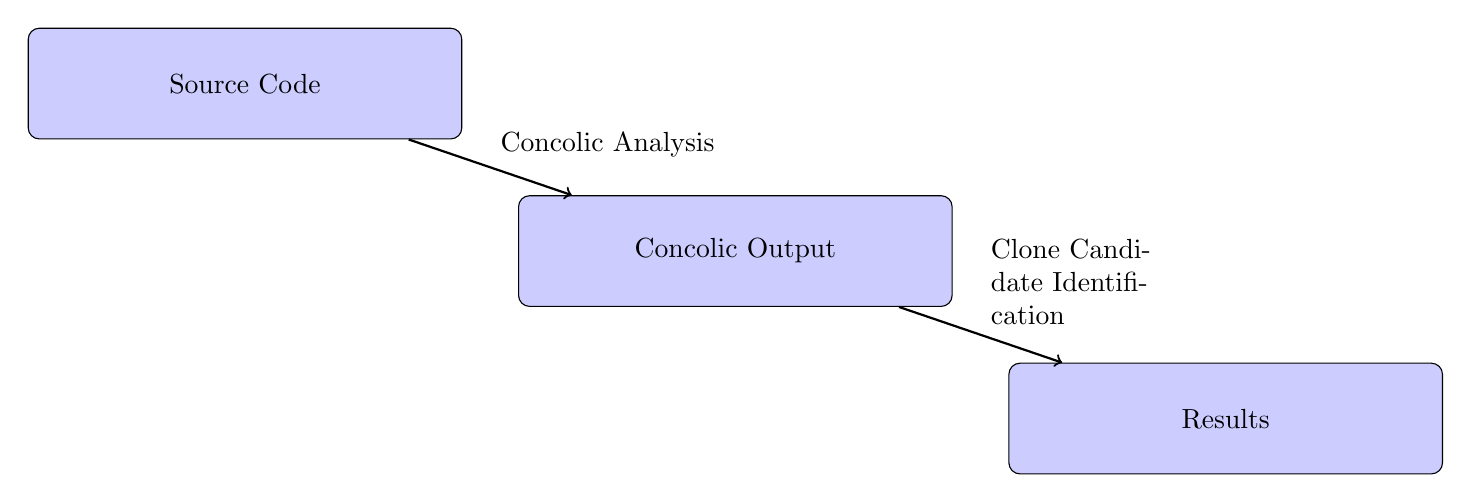
\begin{tikzpicture}[node distance = 2.0cm, auto]

    % Place nodes
	\node [block] (SourceCode) {Source Code};
	\node [block, below right=1.0cm of SourceCode] (ConcolicOutput) {Concolic Output};
	\node [block,  below right=1.0cm of ConcolicOutput] (Results) {Results};
	
	\draw[->] [thick] (SourceCode) to  node {Concolic Analysis} (ConcolicOutput);
	\draw[->] [thick, text width=2.2cm] (ConcolicOutput) to  node {Clone Candidate Identification} (Results);
	
\end{tikzpicture}
\caption{Concolic Analysis}
\label{fig:comprocess}
\end{center}
\end{figure}


Table~\ref{table:royclones} shows two type-4 clones from Roy et al.~\cite{Roy:2009:CEC:1530898.1531101}. These are type-4 clones because code segment \#1 uses a~\emph{for} statement and segment \#2 uses a~\emph{while} statement for looping.


\noindent
\begin{table}[h] %h for here, t for top, b for bottom
\centering
\caption{Example Type-4 Clone from Roy~\cite{Roy:2009:CEC:1530898.1531101}~\label{table:royclones}}
\begin{tabular}{ p{3.8cm} | p{3.8cm} }
\multicolumn{1}{c}{\textbf{Code Segment \#1}} & \multicolumn{1}{c}{\textbf{Code Segment \#2}} \\ \hline \hline
\begin{lstlisting}
void sumProd(int n){
float prod=1.0;
float sum=0.0; //C1
for(int i=1;i<n;i++)
{
    sum=sum + i;
    prod = prod * i;
    foo(sum, prod);
}}
\end{lstlisting}
&
\begin{lstlisting}
void sumProd(int n){
float sum=0.0; //C1
float prod=1.0;
int i=0;
while(i<n)
{
    sum=sum + i;
    prod = prod * i;
    foo(sum, prod);
    i++ ;
}}
\end{lstlisting}
\end{tabular}
\end{table}

Due to space limitations, only a portion of the concolic output from running JPF on these clones is shown in Table~\ref{table:concolicoutputcomparision}. In this example, constant variable types are represented generically by ``CONST'' while the variable type integer is represented by a generic tag ``SYMINT.'' Though not present in this example, other variable types are represented in a similar fashion in concolic output. Actual variable names do not appear anywhere in the output and are irrelevant to the proposed clone detection process. Concolic analysis explores the possible paths that an application can take, with similar execution paths signifying analogous functionality and is thus are indicative of a code clone candidate. Clones in~\emph{dead code} or code that is unreachable via execution paths will not be analyzed by concolic analysis, and therefore are not discoverable via concolic analysis.

\noindent
\begin{table}[h] %h for here, t for top, b for bottom
\caption{Diff of Type-4 Clone Concolic Output}
~\label{table:concolicoutputcomparision}
\centering
\begin{tabular}{ p{3.8cm} | p{3.8cm} }
\multicolumn{1}{c}{\textbf{Concolic Segment \#1}} & \multicolumn{1}{c}{\textbf{Concolic Segment \#2}} \\ \hline \hline
\begin{lstlisting}[style=ConcolicOutput]
### PCs: 1 1 0
original pc # = 1
CONST_`1`<=a_1_SYMINT
SPC#0=
originalPC # = 1
CONST_`1`<=a_1_SYMINT
SPC # = 0
concolicPC # = 0
SPC # = 0
simplePC # = 1
CONST_`1`<=a_1_SYMINT
SPC # = 0
solving: PC # = 1
CONST_`1`<=a_1_SYMINT
SPC # = 0
 --> # = 1
CONST_`1`<=a_1_SYMINT
SPC # = 0 -> true
### PCs: 2 2 0
\end{lstlisting}
&
\begin{lstlisting}[style=ConcolicOutput]
### PCs: 1 1 0
original pc # = 1
CONST_`0`<=a_1_SYMINT
SPC#=0
originalPC # = 1
CONST_`0`<=a_1_SYMINT
SPC # = 0
concolicPC # = 0
SPC # = 0
simplePC # = 1
CONST_`0`<=a_1_SYMINT
SPC # = 0
solving: PC # = 1
CONST_`0`<=a_1_SYMINT
SPC # = 0
 --> # = 1
CONST_`0`<=a_1_SYMINT
SPC # = 0 -> true
### PCs: 2 2 0
\end{lstlisting}

\end{tabular}

\end{table}


In the concolic output in Table~\ref{table:concolicoutputcomparision}, the only differences in these compared segments are the counter values used with the~``CONST'' variable types used in each portion of concolic output. These differences are highlighted in the example.

In order to measure the similarity between sets of the concolic output, the Levenshtein distance measurement is used. This is the minimal number of characters that would need to be replaced to convert one string to another. As an example, if the strings ``ABCD'' and ``BCDE'' are measured, the Levenshtein distance would be 2, because ``A'' would need to be removed and ``E'' inserted into the first string to make them identical. This technique was selected for several reasons, including the impracticality of other string similarity techniques. The Hamming technique, for example, may only be used with strings which are the same length~\cite{Ros:2005:PRR:1086297.1086311, Jain:2012:HES:2324796.2324820}, and concolic output of even two very similar methods rarely yields output of identical length. The longest common subsequence technique does not account for the substitution of values, only the addition and deletion of characters~\cite{Li:2008:SEA:1593105.1593164}.

Because of the relative flexibility of the Levenshtein distance metric, it has proven to be especially well suited for our proposed technique. This is due in part to its ability to work with strings of different lengths and its restriction of upper and lower bounds in the calculated distances. Our distance measurement is achieved using the equation $ALV = (LD/LSL) \times 100$. The Average Levenshtein Value (ALV) is computed by dividing the Levenshtein Distance between two files (LD) by the Longest String Length (LSL) of the two strings being compared and then multiplying by 100. While only a portion of the concolic output is shown in Table~\ref{table:concolicoutputcomparision}, the Levenshtein distance between the two complete sets of output was 25, and the longest string length was 2,216. This means that our formula to calculate the Levenshtein distance between this output is: $ALV = (25/2216) \times 100 = 1.13$, which indicates a very high similarity score, and thus a strong likelihood of a code clone.


We use a Levenshtein threshold score of 30 in our analysis to identify if two compared items are code clones. Our first step in determining this to be the most appropriate Levenshtein value was to use was to produce concolic output from the oracles by Krawitz~\cite{Kraw2012}, Roy~et al.~\cite{Roy:2009:CEC:1530898.1531101} and Krutz and Le~\cite{Krutz:2014:CCO:2597073.2597127} using Levenshtein scores of 0-40 with 10 point increments as a basis for determining clones. To obtain the optimal number, we compared the precision, recall, F-score, and accuracy scores of each increment and found that for all of the code bases, the Levenshtein value of 30 produced the best rates.

We combined the precision, recall, F-score and accuracy values of the code bases and placed them into two charts to better visualize the effects of using the different Levenshtein scores to determine clones. Figure~\ref{fig:levencontrol} displays the results of various Levenshtein values in discovering clones in a single class as defined by Krawitz and Roy~et al. Figure~\ref{fig:levenopen} shows a similar analysis the results from the Krutz and Le~\cite{Krutz:2014:CCO:2597073.2597127} oracle.

%  Krawitz~\cite{Kraw2012}, Roy~et al.~\cite{Roy:2009:CEC:1530898.1531101} and Krutz and Le~\cite{Krutz:2014:CCO:2597073.2597127} 


\begin{center}

\begin{tabular}{lp{2cm}}
\resizebox {\columnwidth} {!} {
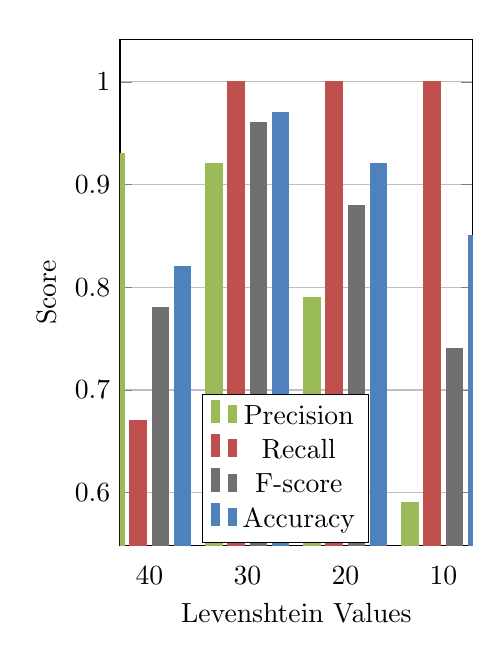
\begin{tikzpicture}
    \begin{axis}[
        width  = .5*\textwidth,
        height = 8cm,
legend style={at={(0.47,0.3)},anchor=north},
        major x tick style = transparent,
        ybar,
        bar width=6pt,
        ymajorgrids = true,
	xlabel={Levenshtein Values},
	ylabel = {Score},
        symbolic x coords={40,30, 20, 10},
        xtick = data,
        scaled y ticks = false,
    ]


       \addplot[style={ggreen,fill=ggreen,mark=none}] % Precision
           coordinates {(40, .93) (30,.92)(20,.79)(10,.59)};

      \addplot[style={rred,fill=rred,mark=none}] % Recall
             coordinates {(40, .67) (30,1)(20,1)(10,1)};

     \addplot[style={ggrey,fill=ggrey,mark=none}] % F-score
           coordinates {(40, .78) (30,.96)(20,.88)(10,.74)};

        \addplot[style={bblue,fill=bblue,mark=none}] % Accuracy
            coordinates {(40, .82) (30,.97)(20,.92)(10,.85)};


     \legend{Precision,Recall, F-score, Accuracy}

    \end{axis}

\end{tikzpicture}
}
\end{tabular}
 \captionof{figure}{Levenshtein Impact In Single Class}
\label{fig:levencontrol}
\end{center}



\begin{center}
\begin{tabular}{lp{2cm}}
\resizebox {\columnwidth} {!} {
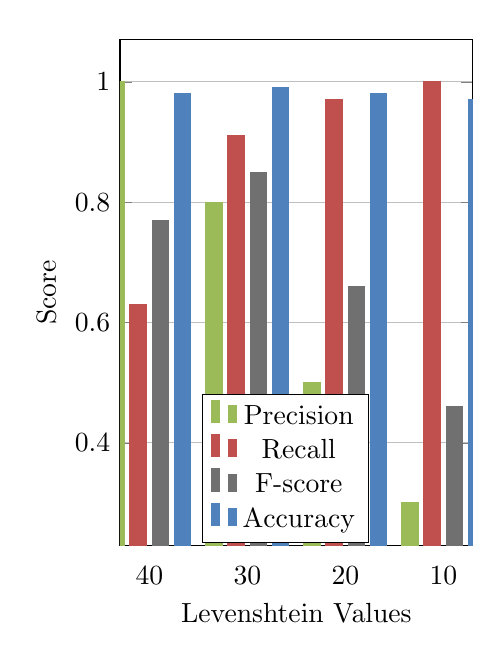
\begin{tikzpicture}
    \begin{axis}[
        width  = .50*\textwidth,
        height = 8cm,
legend style={at={(0.47,0.3)},anchor=north},
        major x tick style = transparent,
        ybar,
        bar width=6pt,
        ymajorgrids = true,
	xlabel={Levenshtein Values},
	ylabel = {Score},
        symbolic x coords={40,30, 20, 10},
        xtick = data,
        scaled y ticks = false,
    ]



       \addplot[style={ggreen,fill=ggreen,mark=none}] % Precision
           coordinates {(40, 1) (30,.8)(20,.5)(10,.3)};

        \addplot[style={rred,fill=rred,mark=none}] % Recall
             coordinates {(40, .63) (30,.91)(20,.97)(10,1)};


   \addplot[style={ggrey,fill=ggrey,mark=none}] %F-score
           coordinates {(40, .77) (30,.85)(20,.66)(10,.46)};

             \addplot[style={bblue,fill=bblue,mark=none}] % Accuracy
            coordinates {(40, .98) (30,.99)(20,.98)(10,.97)};

     \legend{Precision,Recall, F-score, Accuracy}

    \end{axis}

\end{tikzpicture}
}
\end{tabular}
  \captionof{figure}{Levenshtein Impact On Oracle by Krutz and Le~\cite{Krutz:2014:CCO:2597073.2597127}}
\label{fig:levenopen}
\end{center}
 
A higher Levenshtein threshold score is likely to discover more clones, but will also lead to more false positives, creating high precision but lower recall. Conversely, a lower Levenshtein threshold score will find fewer actual clones, but also have less false positives leading to high recall, but low precision. This is because a higher Levenshtein score means that the similarity threshold for noting cloned items will be reduced. A user may select different Levenshtein values depending on their desired levels of precision, recall, F-score and accuracy.

%These findings are important for several reasons. In both examples, the most appropriate Levenshtein score for attaining the highest accuracy, recall and precision was found to be 30, and this value has been used throughout our analysis. Additionally, these findings are indicative of those that future researchers may expect when using concolic analysis to find clones in their respective applications. In certain situations, researchers may wish to increase the recall or precision of their clone discovery technique, using resulting data to seek the most appropriate values.


%\subsection{Preliminary Experiments}

%\todo{make sure to reference this in introduction}

%A simple initial analysis to determine the effectiveness of concolic analysis in code clone detection was done using a type-3 clone as defined by Roy~et al.~\cite{Roy:2009:CEC:1530898.1531101} and is shown in Table~\ref{table:roy_type3}. Concolic analysis was able to detect this clone because it only analyzes the functional nature of the software. The syntactic variations of the two methods which may cause problems for text and syntax-base clone detection tools do not adversely affect the ability of concolic analysis to detect clones.

%\noindent
%\begin{table}%[t] %h for here, t for top, b for bottom
%\centering
%\caption{An Example of Type 3 Clones from Roy~et al.~\label{table:roy_type3}}
%\begin{tabular}{ p{3.8cm} | p{3.8cm} }
%\multicolumn{1}{c}{\textbf{ Code Segment \#1}} & \multicolumn{1}{c}{\textbf{Code Segment \#2}} \\ \hline \hline
%\begin{lstlisting}
%void sumProd1(int n) {
% double sum=0.0;
% double prod=1.0;
% int i;
% for (i=1; i<=n; i++){
%   sum=sum + i;
%   prod = prod * i;
%   foo2(sum, prod);
% }
%}
%\end{lstlisting}
%&
%\begin{lstlisting}
%void sumProd3(int n) {
% double sum=0.0;
% double prod =1.0;
% int i;
% for (i=1; i<=n; i++){
%  if (i %2 == 0){
%   sum+= i;
%  }
% prod = prod * i;
% foo2(sum, prod);
% }
%}
%\end{lstlisting}

%\end{tabular}
%\end{table}


\section{Evaluation}
\label{sec: evaluation}


In the following sections, concolic analysis for clone detection will be evaluated against two small oracles created by Krawitz~\cite{Kraw2012} and Roy~et al.~\cite{Roy:2009:CEC:1530898.1531101} and a larger oracle built by Krutz and Le~\cite{Krutz:2014:CCO:2597073.2597127} to determine what types of clones concolic analysis is capable of finding, along with its accuracy, precision, recall and F-score.



\subsection{Types of Clones Discovered} %% Give a better Title?


%%% I removed this section because I wanted to remove the analysis using Java. I felt like it opened too many potential holes for people to attack us through.

%Our Java-based prototype used Java Path Finder (JPF) to produce the concolic output of the target application. Unfortunately, due to technical limitations of the tool, we were unable to analyze any reasonably sized open source applications using JPF. Of the most profound was its inability perform concolic analysis on several variable types including float, byte, and short, significantly limiting the amount of methods JPF was able to analyze. Without further development, continued use of this tool would have led to inaccurate results since such a large number of methods would have had to been ignored or allowed to produce errors during concolic analysis. Because of this, the Java implementation will only examine proof of concept classes and will not analyze the more complicated Java-based open source applications or similar-sized code bases.

The C-based applications were analyzed by concolic analysis using the \ifisnopii Concolic Code Clone Detection (CCCD) tool which we published in a previous work~\cite{wcre2013}.\else xxxx tool, which we published in a previous work[citation removed]. \fi In the previous paper, we demonstrated the ability of concolic analysis to effectively discover all types of code clones in a very small environment but did not thoroughly analyze the technique. We will build on these results and further evaluate concolic analysis for clone detection. \\

% using a larger oracle.
%compare concolic analysis against several leading existing clone detection tools using clones as defined in previous research by Krawitz~\cite{Kraw2012} and Roy~et al.~\cite{Roy:2009:CEC:1530898.1531101}. \\


\textbf{RQ1: \emph{What types of clones is concolic analysis effective at detecting?}}
The initial step of evaluating concolic analysis for code clone detection was to evaluate it against 4 clones defined by Krawitz, and 16 by Roy et al. These 20 defined clones were added to a single Java and C file. The results in Table~\ref{table:singleclasscomparisionexample} indicate the ability of concolic analysis to find a wide range of clones in this small, controlled environment in both C and Java applications. We used \ifisnopii CCCD \else xxxx \fi for the C code, and developed a small prototype based upon JPF for the Java code.


\begin{table}[thb!]
\begin{center}
\caption{Concolic Analysis Finding Clones on Single Class}
\label{table:singleclasscomparisionexample}
\begin{tabular}{r||l|l|l|l|l}
\bfseries Language & \bfseries T1 & \bfseries T2 & \bfseries T3 & \bfseries  T4 & \bfseries  Total \\ \hline\hline
 \bfseries  Java  & 5 & 6 & 6 & 6  & 23 (96\%)\\
  \hline
\bfseries  C  & 5 & 6 & 7 & 4  & 22 (92\%)\\

  \hline
\bfseries Total Possible & 5 & 6 & 7 & 6 & 24 \\ %\hline

\end{tabular}

\end{center}
\end{table}


Within the limited Java implementation, the concolic analysis based technique was able to detect 96\% of all clones. The only clone which concolic analysis was unable to detect was a type-3 clone as defined by Roy~et al. since JPF was unable to traverse all paths of this method for technical reasons, including its inability to perform analysis on several unsupported variable types (float, byte, and short). This limitation ultimately affects the concolic analysis clone identification process specifically when applied to Java. A similar C file containing the clones of Krawitz and Roy~et al. was then examined for clones. 

In the example, concolic analysis was able to detect 92\% of all clones. The only clones that concolic analysis was unable to detect were the type-4 clones as defined by Krawitz. In this clone example, a method has been refactored into two functionally similar methods. Two different concolic paths were generated for these methods, and thus the generated concolic output was not similar, so no clone code candidate was detected. Our technique did however find all other instances of type-4 clones. The size of the examined functions did not have a significant impact on the ability of any of the examined processes in detecting clones.

This small example demonstrates that concolic analysis for code clone detection is capable of finding all four types of clones in both Java and C. \\




\subsection{Effectiveness of Concolic Analysis For Code Clone Detection}
\label{sec: acc_prec_rec}

Our next step was to evaluate the effectiveness of code clone detection in terms of precision, recall, F-score, and accuracy. \\  

% make this not be from Kruz & Le in final version
\textbf{RQ2:~\emph{How effective is concolic analysis for code clone detection?}}\\
In order to evaluate the effectiveness of concolic analysis for code clone detection, we used a function level clone oracle created by Krutz and Le~\cite{Krutz:2014:CCO:2597073.2597127} since it is the only known oracle to contain all four types of code clones explicitly defined. We ran concolic analysis for code clone detection and measured the accuracy, precision, recall, and F-score of this technique against this clone oracle.

The oracle was created by first randomly selecting 3-6 classes from Apache, Python, and PostgreSQL. A specially made comparison tool allowed several researchers to independently manually compare all functions and record if the compared functions were code clones, and if so what type of clone they were. Several leading clone detection tools were then ran against the code base with their findings being recorded. These tool results were then used by the researchers to identify any clones which they may have missed for further analysis. However, the ultimate decision of whether or not two compared functions represented a clone fell upon the researchers and not any tool. When researchers disagreed if two compared functions represented, or on the type of clone, a discussion took place until a consensus could be reached. \ifisnopii While CCCD was one of the selected tools used as input for this oracle, since all clone decisions were manually verified and tools were never the deciding factor as to what constituted a clone, we do not feel like this negatively impacted the results. \else \fi

Precision, recall, F-score and accuracy are important factors in evaluating clone detection tools~\cite{Zibran:2012:IRF:2231936.2231970}. They should not return too high of a rate of false positives, but also not miss a significant portion of code clones. The definitions we used for precision, recall, F-score and accuracy are described below:

 \begin{enumerate}
  \item~\textbf{Precision:} Ratio of the clone pair which a tool reports that are true clones, not false positives. % Relates the number of files predicted~\emph{and} observed as defect prone to the number of files predicted as defect prone. It is calculated as $\frac{a}{a+b}$.

 \item~\textbf{Recall:} Ratio of the clone pairs in a system that a tool is able to detect. %Relates the number of files predicted~\emph{and} observed as defect prone to the number of files that actually had defects. It is calculated as $\frac{a}{a+c}$.

  \item~\textbf{F-score:} Considers precision~\emph{and} recall to measure the accuracy of a system. It is calculated as $2\times(\frac{precision\times recall}{precision+recall})$. Sometimes referred as F1 or F-measure.

 \item~\textbf{Accuracy:} Percentage of elements classified correctly. The highest attainable value is 1.0. %It is calculated as $\frac{a+d}{a+b+c+d}$.

\end{enumerate}



%%%% \cite{Lin:2014:DDA:2568225.2568298}


 %To study the prediction accuracy, we built two multivariate logistic regression models: one that uses all of the metrics and one that uses a smaller set of statistically and minimally collinear metrics. The logistic regression models are designed predict the likelihood of a file being defect prone or otherwise. The output is given as a value between 0 and 1; we classified values above 0.5 as defect prone, with the remainder classified defect free. The classification results of the prediction models were stored in a confusion matrix, as shown in Table~\ref{Table:conf_matrix}. \todo{fix this}
%\begin{table}[h!]
%  \centering
%\caption{Confusion matrix}
%\label{Table:conf_matrix}
%  \begin{tabular}{cc|cc}
%    & &\multicolumn{2}{c}{\textbf{True  Class}} \\
%    \cmidrule(rl){3-4}
%    & & Yes & No \\
%    \hline
%    \multirow{2}{*}{\textbf{Predicted}}
%    & Yes & a & b \\
%    & No & c & d \\
%    \hline
%  \end{tabular}
%\end{table}


%The performance of the prediction model is measured in four different ways. Values for each will range from 0 to 1, with a 1 being favorable:
%\begin{enumerate}
%  \item~\textbf{Precision:} Relates the number of files predicted~\emph{and} observed as defect prone to the number of files predicted as defect prone. It is calculated as $\frac{a}{a+b}$.

 % \item~\textbf{Recall:} Relates the number of files predicted~\emph{and} observed as defect prone to the number of files that actually had defects. It is calculated as $\frac{a}{a+c}$.

 % \item~\textbf{F-Score:} Considers precision~\emph{and} recall to measure the accuracy of a system. It is calculated as $2\times(\frac{precision\times recall}{precision+recall})$. Sometimes referred as F1 or F-measure,

% \item~\textbf{Accuracy:} Percentage of elements classified correctly. The highest attainable value is 1.0. It is calculated as $\frac{a+d}{a+b+c+d}$.

%\end{enumerate}









In order to evaluate the effectiveness of concolic analysis for clone detection against an existing technique, we compared \ifisnopii CCCD \else xxxx \fi against MeCC, a tool which is capable of discovering all four types of code clones~\cite{Kim:2011:MMC:1985793.1985835}. We ran MeCC against the Krutz and Le~\cite{Krutz:2014:CCO:2597073.2597127} oracle using a variety of values for its two input parameters, similarity, and minimum entry size. We used the settings which produced highest rates of precision, recall, accuracy, and F-score values against the clone oracle which were a similarity of 80 and a minimum line entry of 4. We then ran \ifisnopii CCCD \else xxxx \fi against the same oracle. The resulting averages for each tool are shown in Table~\ref{Table:precisionrecall}.




%%% Just provided the averages since the .06 for p-SQL and MeCC looked very bad

%\begin{table}[thb!]
%\begin{center}
%\caption{Precision, Recall, F-Score \& Accuracy for Each Tool}
%\label{Table:precisionrecall}
%\begin{tabular}{r||l|l|l|l|l}
%\bfseries Tool & \bfseries Example & \bfseries Precision & \bfseries Recall & \bfseries F-Score & \bfseries Accuracy \\ \hline\hline
%\bfseries Mecc & \bfseries Apache & .94 & .52 & .67 & .95 \\ \cline{2-6}
%& \bfseries P-SQL & .06 & .4 & .1 & .95 \\ \cline{2-6}
%& \bfseries Python & .8 & .5 & .62 & .97 \\ \cline{2-6}
%& \bfseries avg. & .6 & .47 & .46 & .96 \\ \cline{2-6}
% \hline \hline
%\bfseries CCCD & \bfseries Apache & 1 & .9 & .95 & .99 \\ \cline{2-6}
%& \bfseries P-SQL & .73 & .96 & .83 & .98 \\ \cline{2-6}
%& \bfseries Python & .67 & .84 & .75 & .98 \\ \cline{2-6}
%& \bfseries avg. & .83 & .93 & .88 & .98 \\
%\end{tabular}

%\end{center}

%\end{table}




\begin{table}[thb!]
\begin{center}
\caption{Average Precision, Recall, F-Score \& Accuracy}
\label{Table:precisionrecall}
\begin{tabular}{l|l|l|l|l}
\bfseries Tool & \bfseries Precision & \bfseries Recall & \bfseries F-Score & \bfseries Accuracy \\ \hline\hline
 \bfseries MeCC & .6 & .47 & .46 & .96 \\ \cline{2-5}
 \hline
 \bfseries \ifisnopii CCCD \else xxxx \fi & .8 & .91 & .85 & .99 \\
\end{tabular}

\end{center}

\end{table}


These results demonstrate the effectiveness of concolic analysis for clone detection against a leading tool. While both techniques are able to achieve a high rate of accuracy, \ifisnopii CCCD \else xxxx \fi has a much higher F-score and recall than MeCC.




%\begin{table}[thb!]
%\begin{center}
%\caption{Concolic Analysis for Clone Detection Rates}
%\vspace{0.1in} % Add a small buffer between title and table
%\label{Table:precisionrecall}
%\begin{tabular}{l|l|l|l|l}
%\bfseries Oracle Example & \bfseries Precision & \bfseries Recall & \bfseries F-Score & \bfseries Accuracy \\ \hline\hline
%\bfseries Apache & 1 & .9 & .95 & .99 \\ \cline{1-5}
% \bfseries P-SQL & .73 & .96 & .83 & .98 \\ \cline{1-5}
% \bfseries Python & .67 & .84 & .75 & .98 \\ \cline{1-5} \hline\hline
% \bfseries Avg. & \bfseries .83 & \bfseries .93 & \bfseries .88 & \bfseries .98 \\ \cline{1-5}
% \hline %\hline
%\end{tabular}
%\end{center}
%\end{table}

Concolic analysis has been shown to be a powerful clone detection method which is not only able to discover a wide range of clone types (including type-4), but is also able to find them with a high rate of precision, recall, F-score, and accuracy.


%\section{Discussion}
%\label{sec: discussion}

%During our analysis of concolic analysis for clone detection, we found several interesting areas that warrant further discussion. We will present the effects that using various Levenshtein distance values have in determining clones has on the precision, recall, F-score, and accuracy values of concolic analysis for clone detection. Next we will discuss how the Levenshtein score between compared clone candidate functions are relate to the likelihood of different types of clones found by concolic analysis.


%\subsection{Levenshtein Distance}

%% The table values are correct, the chart values are wrong.
%\todo{There are problems with these scores. They values in chart do not match up against the ones in the table}

%\todo{describe the control and krawitz and krutz oracles}


\section{Related Works}
\label{sec: relatedworks}

There are numerous clone detection tools which utilize a variety of methods for discovering clones including text, lexical, semantic, symbolic and behavioral based approaches \cite{Roy:2009:CEC:1530898.1531101,Kim:2011:MMC:1985793.1985835}. However, only a few are known to be able to reliably detect type-4 clones. MeCC discovers clones based on the ability to compare a program's abstract memory states. While this work was successful in finding type-4 clones, there are several areas for improvement such as its limitation in analyzing pre-processed C programs and an excessive clone detection time, likely caused by the exploration of an unreasonably large number of possible program paths~\cite{Kim:2011:MMC:1985793.1985835}. Krawitz~\cite{Kraw2012} proposed a clone discovery technique based on functional analysis which was shown to detect clones of all types, but was never implemented into a reasonably functional tool. This technique also requires a substantial amount of random data, which may be a difficult and time consuming process to produce. There are numerous other clone detection tools which have been used in previous research. Roy et al.~\cite{Roy:2009:CEC:1530898.1531101} carried out a thorough analysis of many tools in 2009 which describes many of the different types of clone detection tools and techniques. Subsequent works have compared tools, but on a smaller scale~\cite{arcelli2013software,svajlenko2013scaling}.

The most prominent area that concolic analysis has been applied to thus far is software testing, specifically for dynamic test input generation, test case generation, and bug detection \cite{Wassermann:2008:DTI:1390630.1390661, Sen:2005:CCU:1081706.1081750}. Several tools exist for performing concolic analysis, including Crest, Java Path Finder, CUTE~\cite{Sen:2005:CCU:1081706.1081750}, and Pex \footnote{\url{http://research.microsoft.com/en-us/projects/pex}}.

We chose to use the code clone oracle created by Krutz and Le~\cite{Krutz:2014:CCO:2597073.2597127} in 2014 since it explicitly contains all four types of code clones, but there are several other prominently used clone oracles which have been proposed in previous research. Tempero~\cite{IWSC13p53} described a collection of 1.3M method-level-clone-pairs from 109 different systems. The goal of this work was to create a similar data set for clone research. While this work was profound, much of the data has a low level of confidence and requires further work and analysis.

Lavoie and Merlo~\cite{Lavoie:2011:ATC:1985404.1985411} created a clone oracle set containing type-3 clones using the Levenshtein metric. There was no mention of type-4 clones in this oracle. Bellon et al.~\cite{4288192} created a robust clone oracle which has been used in a substantial amount of research. This work was recently extended upon by Murakami et al.~\cite{Murakami:2014:DCR:2597073.2597133}. Unfortunately, neither of these oracles contain any explicitly defined type-4 clones.


\section{Threats to validity}
\label{sec: threats}
There are several threats to the validity of our results. First, our results were only run on Java and C. We do not believe the they would significantly differ if concolic clone detection was run in different languages, but without verification it is impossible to tell for certain. Concolic analysis only executes the functional aspects of an application, meaning that it will not be able to detect clones in non-functional portions of the software. This technique is also limited by the concolic analysis tools available for use, and while these tools continue to improve and are robust, they are not perfect. In some cases they are unable to traverse various portions of an application or are incapable of recognizing segments of the software for technical reasons. This inhibits the clone detection process for these portions of the application. Finally, the followed path conditions depend upon the control flow graph and its predicates, meaning that concolic analysis for clone detection is still dependent upon its implementation. While it is less dependent than syntax or token based clone detectors, many code instances of identical semantics or different implementations will not be detected by concolic analysis for clone detection. Concolic analysis may also be a slow, and resource intensive process which could adversely affect an implementation of our technique on a very large code-base.

A significant portion of this study was based off previous research by Krawitz~\cite{Kraw2012}, Roy~et al.~\cite{Roy:2009:CEC:1530898.1531101}, Krutz and Le~\cite{Krutz:2014:CCO:2597073.2597127}, and Kim~et al.~\cite{Kim:2011:MMC:1985793.1985835}. Therefore, our results depend to a certain extent on the benchmarks provided by the aforementioned prior work. Manually finding type-4 clones in source code is extremely difficult and there are only few automated techniques which are known to reliably find type-4 clones. This makes it very difficult to test a new mechanism in finding these clones since there are very few benchmarks to be evaluated against.


The classification of clones and their type is a difficult and imprecise task~\cite{Walenstein:2003:PCT:950792.951349}, so many researchers will likely disagree with the classification of clones from our oracles. This is a problem which is not at all unique to our work and affects other research as well~\cite{Lavoie:2011:ATC:1985404.1985411}. While many works recognize type-4 clones~\cite{Roy:2009:CEC:1530898.1531101,4288192} other recent research does not acknowledge the existence of type-4 clones~\cite{Duala-Ekoko:2010:CRD:1767751.1767754,Lavoie:2011:ATC:1985404.1985411}, so there is some fragmentation in the code clone community as to whether type-4 clones even exist. In spite of these possible limitations, we are confident that concolic analysis is able to discover type-4 clones as is exemplified by our evaluation using our chosen oracles.





%the small sample oracle largely derived from Krawitz~\cite{Kraw2012} and Roy~et al.~\cite{Roy:2009:CEC:1530898.1531101}. Unfortunately, since type-4 clones are very hard to manually identify and are only found by one existing tool, generating an accurate evaluation of a new technique in its ability to accurately identify type-4 clones is very difficult.

%While we did our best to manually identify and classify clones using several people, and previous research has demonstrated the difficulty and problems with manually identifying and classifying code clones~\cite{Walenstein:2003:PCT:950792.951349}. This indicates that other researchers may disagree with many of the clones identified and how they were classified in our work. This is a problem which is not at all unique to our work and is one that hinders other research as well~\cite{Lavoie:2011:ATC:1985404.1985411}.






%There are also numerous clone detection tools that detect clones in numerous different ways. While we were able to compare concolic analysis to several other leading detection processes, it is unreasonable to attempt to compare them to all known techniques. Many clone detection tools have adjustable inputs which may be altered to determine the size of the methods examined for clones, along with the similarity score needed to determine if two methods are defined as clones. While we did our best to use the most appropriate input settings for each tool, it is quite possible that more appropriate settings could have been selected to yield more accurate results. When we were unsure of the most appropriate setting, we chose to use the defaults for each tool.



We compared concolic analysis (using \ifisnopii CCCD \else xxxx \fi) against MeCC and evaluated their rates of precision, recall, F-score and accuracy. One potential problem with this comparison is that MeCC finds clones at the sub method level, while \ifisnopii CCCD \else xxxx \fi is only capable of discovering clones at the method level. In order to mitigate this problem, we analyzed all clones identified by MeCC which were at the method level and used them for our comparison. This means that MeCC will likely discover more clones than \ifisnopii CCCD \else xxxx \fi, but could also lead to more false positives. While we acknowledge that this could create a bias of our findings, the purpose of this comparison was not to state that \ifisnopii CCCD \else xxxx \fi was necessarily better than MeCC, but to merely demonstrate that concolic analysis is a powerful mechanism for clone detection.



% Make it one section
\section{Future Work}
\label{sec: futurework}
While we demonstrated that concolic analysis is capable of reliably and accurately discovering all four types of clones, future work may be conducted in several key areas. We only compared concolic analysis for clone detection against MeCC. Future work should be done comparing our techniques against other leading clone detection tools such as SeByte~\cite{Keivanloo:2012:JBC:2664398.2664404}, CCFinderX~\footnote{\url{http://www.ccfinder.net/ccfinderx.html}}, ConQat\footnote{\url{https://www.conqat.org/}}, ctCompare\footnote{\url{http://minnie.tuhs.org/Programs/Ctcompare/}}, Deckard\footnote{\url{https://github.com/skyhover/Deckard}}, iClones\footnote{\url{http://www.softwareclones.org/iclones.php}}, Simian\footnote{\url{http://www.harukizaemon.com/simian/}}, Simcad\footnote{\url{http://homepage.usask.ca/~mdu535/tools.html}}, and Nicad\footnote{\url{http://www.cs.usask.ca/~croy}}.

We used an oracle created by Krutz and Le~\cite{Krutz:2014:CCO:2597073.2597127} since it contained all four types of clones. We did not choose to use oracles from Bellon et al.~\cite{4288192} or Murakami et al.~\cite{Murakami:2014:DCR:2597073.2597133} since they did not explicitly contain type-4 clones. However, future work may be done to expand on our findings using these oracles. 

%The only fully functional implementation of concolic analysis for clone detection has been implemented in \ifisnopii CCCD~\cite{wcre2013} \else xxxx \fi, which we largely based our research off of and only works with C programs. Future researchers may choose to develop tools capable of analyzing other languages, such as Java.

Finally, we have demonstrated that concolic analysis for clone detection may only discover clones at the method level. Future work can be done to implement a concolic-based solution which may locate clones at a more granular level. The biggest obstacle in creating this solution is with the comparison process that our technique uses for discovering clones. Currently, the concolic output from each method is compared to the others in a round robin fashion. Comparing snippets of code with one another would be a virtually insurmountable task. Future work may be done to develop a more efficient comparison process.


\section{Conclusion}
\label{sec: conclusion}



Concolic code clone detection represents a new and powerful clone detection technique which we have demonstrated to be capable of finding all four types of code clones with high precision, recall, accuracy, and F-score values. We evaluated concolic analysis for clone detection using a small C and Java based oracle, and then with a larger oracle comprised of C code. The proposed clone detection technique is innovative because it not only represents the first known concolic-based clone detection technique, but is also one of only a few known processes which is able to reliably detect type-4 clones.


\balance
\bibliographystyle{abbrv}
\bibliography{concoliccodeclone}  % sigproc.bib is the name of the Bibliography in this case

\balancecolumns
% That's all folks!
\end{document}

%%%% Notes
% 6 pages (2 at extra cost)
% http://selab.uos.ac.kr/sacse15/


%%%% Todo
% Add in General terms?
% Make sure we address all the issues discussed in the EMSE feedback
% There are quite a few references, maybe remove a few of them
% Table and figure labels on top or bottom?
%   F bottom, table top
% Fix figure 1, concolic analysis
% In our system, we used an average Leven distance of X -- meaning that X characters in each were different
%$$$

% Remove some of the unnecessary citations

% After acceptance
%   Change wording say us, not Krutz
%
